\chapter{Beginning to Decode}

\section{Instruction Decode}

The next stage in the datapath is the iDecode stage.  The iDecode stage evaluates the binary instructions (an output of the iFetch stage) and determines what needs to be done.  There are many aspects to the iDecode stage, and some get fairly complex.  But today we will begin the process of decoding that instruction by decomposing the instructions into the key parts of R-Type and D-Type instructions:
\begin{enumerate}
	\item Opcode
	\item Address (used only in D-Type instructions)
	\item Rm (used only in R-Type instructions)
	\item Rn
	\item Rd (though the book uses Rt for D-type instructions, we will use Rd for the last operand of D-type instructions)
\end{enumerate}   

To do this, you will create a new module called instr\_parse.  This module will simply read inputs and assign appropriate output values.  These outputs should be assigned on the clock edge with non-blocking procedural assignments.  While this might not seem important now, it will become important later.  The inputs should be a clk signal and a 32-bit instruction.  Outputs are listed for you above.  Although R-type and D-type instructions have different operands, you can treat them the same for now.  For instance, you can still assign an Address field on an R-type instruction, and you can still assign an Rm field on a D-type instruction.  In future labs, we will begin treating the instructions differently and ignore the unnecessary fields.  Notice how because of the commonality of instruction format, Opcode, Rn, and Rd are all universal across these instruction types.  Please remember to use the style specified in the previous lab, where all items are lower case with underscores separating them.  For instance, for Rd, you should use the signal name rd\_num.  Appending num on the end of the name indicates that this is the register number, not the value from the register.

To test this, you will need to create an instr\_parse\_test.v that will feed the module with a clock signal and instructions.  Then you can verify that your instructions are being parsed correctly.

\section{Register File}

Next, we will create the register file.  You will create a new module called regfile (in regfile.v).  The regfile module should retrieve data from the registers on the rising edge of read\_clk as well as write to the registers on the rising edge of write\_clk when the regWrite flag is set.  The regfile should use a verilog reg array.  You do not need to use the register module that you used for your program counter.  Since we don't currently have the ability to do loads and stores (since we don't have data memory yet), the values for the registers should be stored in a datafile, regData.data and read in during the initial block, just like we did with the instr\_mem.v file.  

Inputs to the module should include a signal called read\_clk and a signal called write\_clk as well as all inputs shown on the Register file in Figure~\ref{fig:register_file_cutout}.  The outputs should be the outputs of the Register file in Figure~\ref{fig:register_file_cutout}.  Use names such as read\_register1, read\_data2, etc.

You will need to write a testbench, regfile\_test.v, for this module as well.  It should provide values for each input and verify that the outputs match expected behavior.

\begin{figure}
	\caption{Expected Results}\label{fig:register_file_cutout}
	\begin{center}
		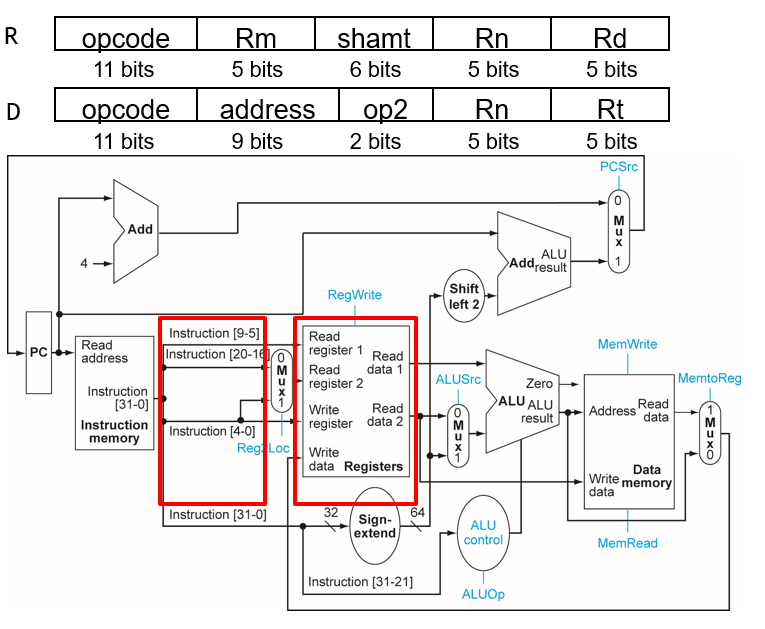
\includegraphics[width=4.75in]{../images/register_file_cutout.png}
	\end{center}
\end{figure} 


\clearpage
\section{Your Assignment}

You are to:
\begin{enumerate}
\item Create an instr\_parse module as described above.
\item Create an instr\_parse test module and verify that the instruction is being parsed properly.
\item Create a regfile module as described above.
\item Create a regfile\_test module and verify that the values are being stored and retrieved from the regfile properly.
\end{enumerate} 